\section{Laser module}

\subsection{Laser}
The laser plays one of the key role in the whole system.
Strict requirements are imposed on it, starting from the pulse energy, ending with the generation stability. 
The maximum distance at which we can detect an object directly depends on the pulse energy, in our case the energy should be more than 1uJ to reach 200m distance.
To get a picture in good pixel resolution, especially at high FPS, we need a fairly fast pulse repetition rate, at least 10kHz.
Using the TOF method it is extremely important to have a small pulse width, the smaller, the smaller the measurement error and the higher the accuracy.
To obtain acceptable accuracy, the pulse width should be less than 10 ns and have a Gaussian-like shape, moreover timing jitter should be as small as possible.
The wavelength of the laser should coincide with the receiver spectrum for better amplification, in the case of SiPM it is around 420 nm.
Being used in space, reability, size and power consumption become critical.

Finaly, the requriments for laser is: \\


\begin{table}[H]
\label{tbl:rfp_laser}
\begin{center}

\begin{tabular}{|p{0.2\linewidth}|p{0.3\linewidth}|}
\hline
Pulse energy: & \textbf{$\geq$ 1 uJ}  \\ \hline
Repetition rate: & \textbf{$\geq$ 10 kHz} \\\hline
Pulse duration: & \textbf{$\leq$ 10 ns} \\\hline
Wavelength, $\lambda$: & \textbf{depends on SNR, <1000nm} \\\hline
Power consumption: & \textbf{$\leq$ 2 W} \\  \hline
Dimension: & \textbf{$\leq$ 3 cm$^3$} \\  \hline
\end{tabular}
\caption{Requirements for the laser system}
\end{center}
\end{table}


Nowadays, there are a lot of laser solutions: Solid-state lasers, Semiconductor lasers, Fiber lasers, Gas lasers, but many of them do not meet all our requirements.
Solid-state lasers can be used in a pulsed mode with Q-switching (active or passive) technique and also in Mode-locking mode. In the case of the Mode-locking mode, the repetition frequency can reach many MHz, whereas the pulse duration is much lower: typically between 30 fs and 30 ps. Despite the complexity of creation such laser, the energy of the pulse, is extremely small and can not be used for our purposes.


\begin{figure}[H]
\begin{minipage}[h]{0.52\linewidth}
\center{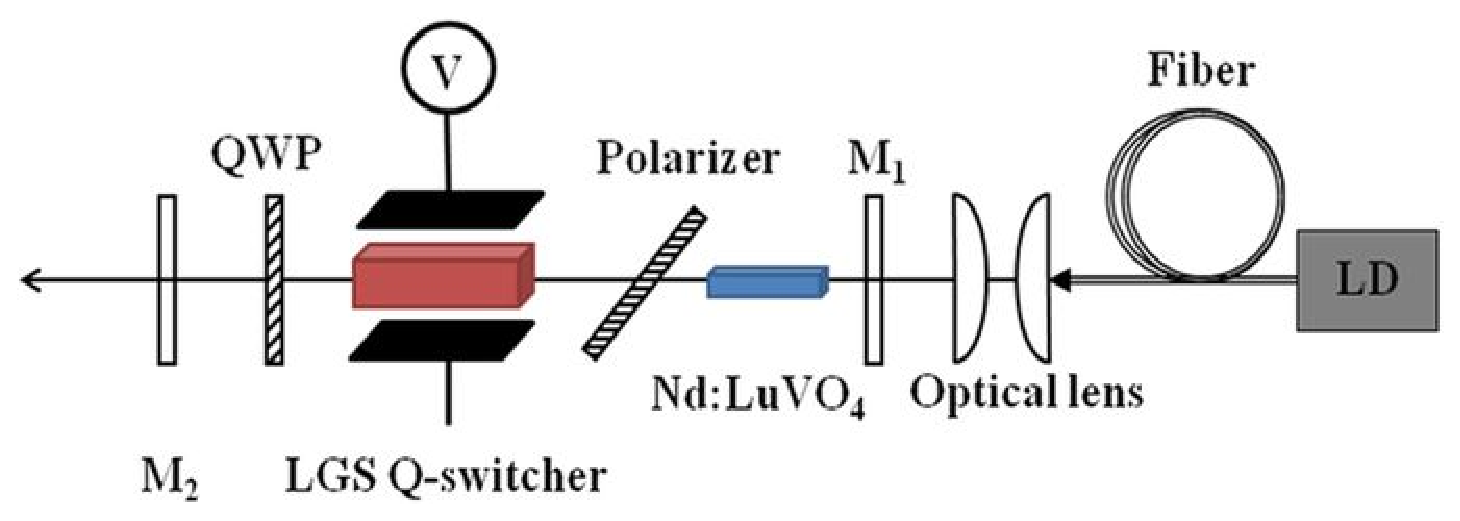
\includegraphics[height=3.25cm, width=1\linewidth]{act_q}} a) \\
\end{minipage}
\hfill
\begin{minipage}[h]{0.45\linewidth}
\center{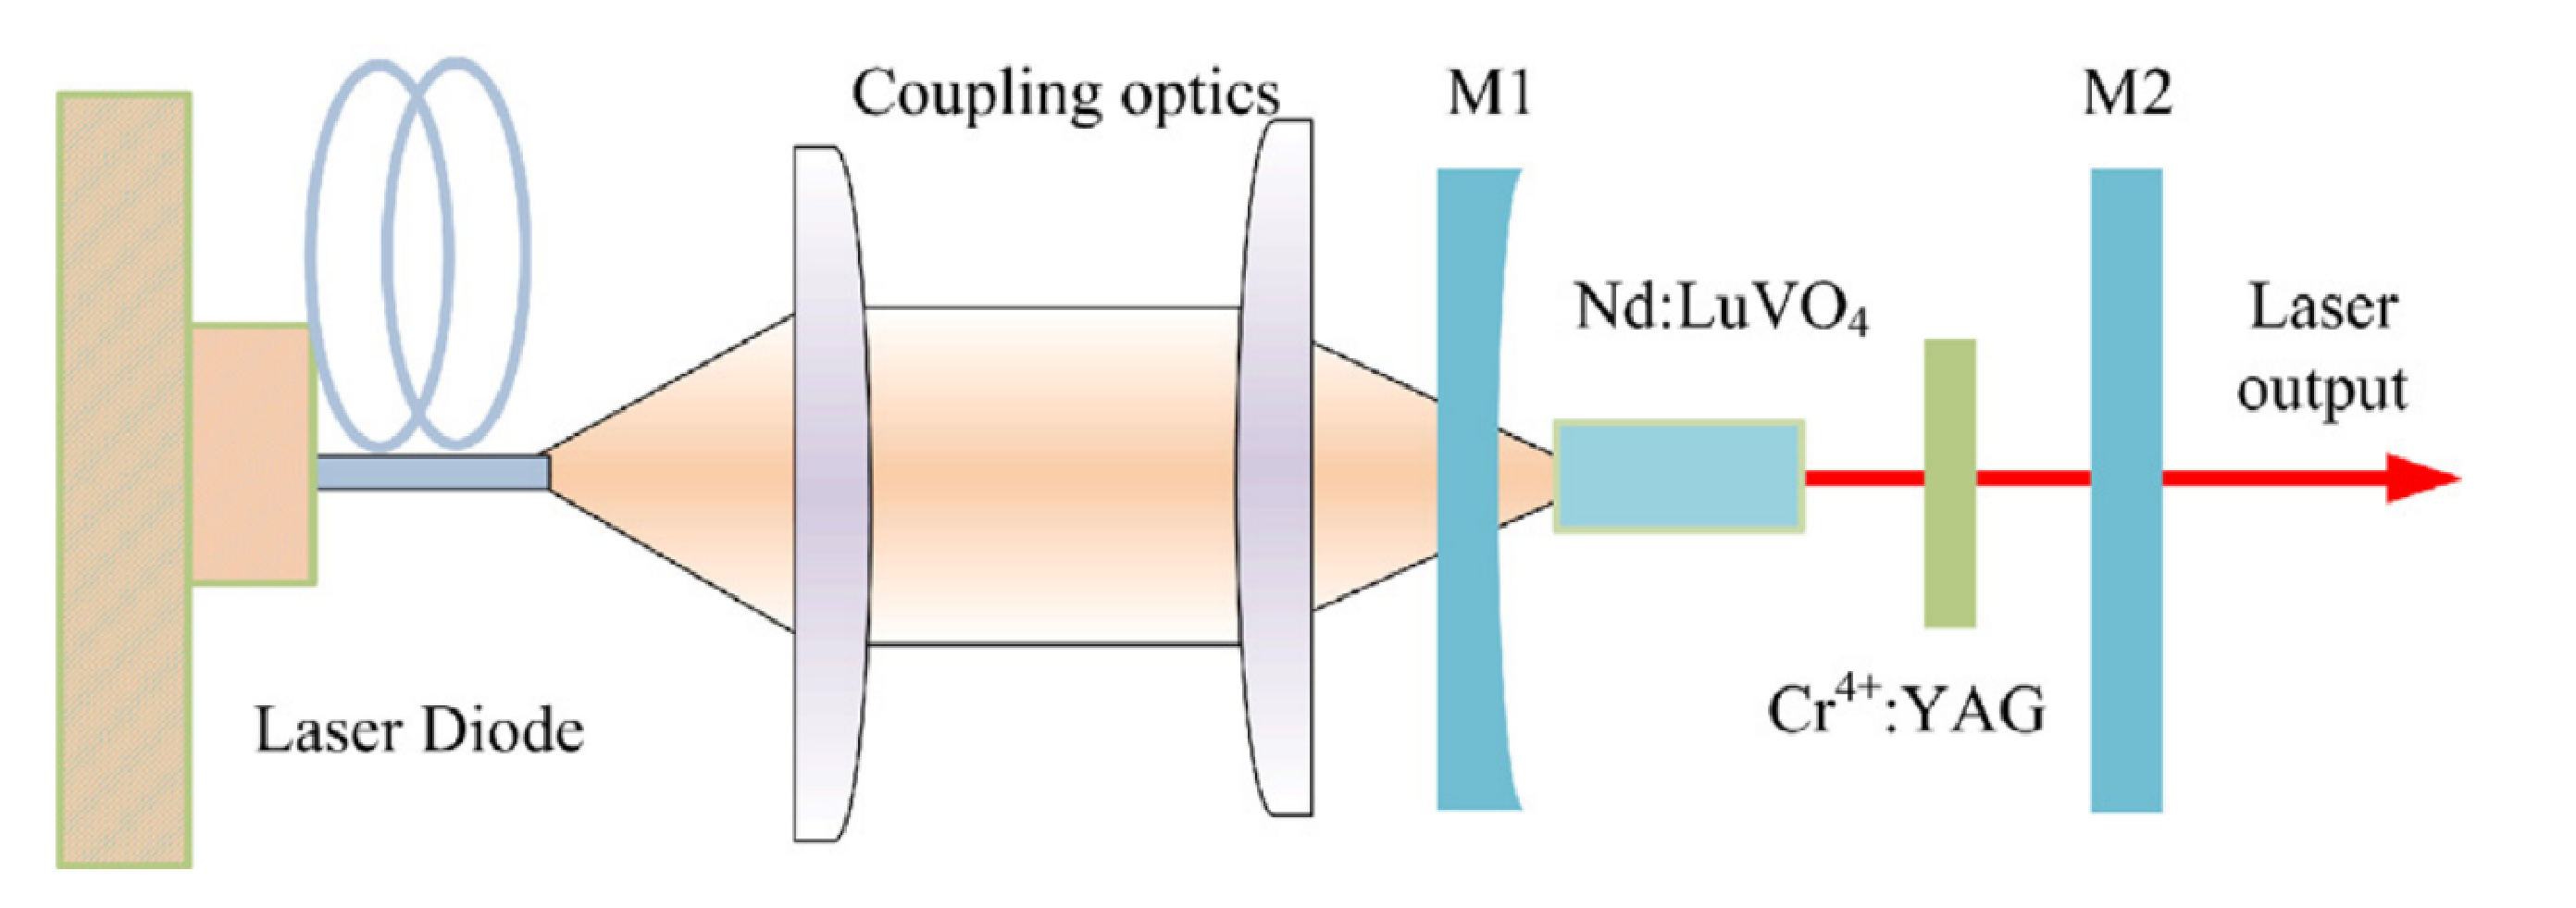
\includegraphics[height=3.05cm, width=1\linewidth]{pas_q}} \\b)
\end{minipage}


\caption{Typical Q-switched schemes for active and passive mode:
a) Laser diode end-pumped activelly Q-switched laser utilizing a langasite (LGS) crystal as an electro-optic Q-switch.
b) High repetition rate laser-diode end-pumped passively Q-Switched Nd:LuVO4/Cr4+:YAG
}
\label{fig:qs_lasers}
\end{figure}

In case of Q-switched lasers (Fig. ~\ref{fig:qs_lasers}), the pulse repetition rate is typically in the range from 1–100 kHz, sometimes higher. Passively Q-switched microchip lasers have reached pulse durations far below 1 ns and repetition rates up to several megahertz, whereas large (typically amplified) laser systems can deliver pulses with many kilojoules of energy and durations in the nanosecond range. For active Q-switching, the losses are modulated with an active control element (active Q-switch), typically either an acousto-optic or electro-optic modulator. Here, the pulse is formed shortly after an electrical trigger signal arrives. There are also mechanical Q-switches such as spinning mirrors, used as end mirrors of laser resonators. In any case, the achieved pulse energy and pulse duration depends on the energy stored in the gain medium, i.e. on the pump power and the pulse repetition rate.
For passive Q-switching (sometimes called self Q-switching), the losses are automatically modulated with a saturable absorber.
Here, the pulse is formed as soon as the energy stored in the gain medium (and thus the gain) has reached a sufficiently high level. In many cases, the pulse energy and duration are then fixed, and changes of the pump power only influence the pulse repetition rate.
Compared with active Q-switching, passive Q-switching is simple, takes up little space and cost-effective (eliminating the modulator and its electronics), and is suitable for very high pulse repetition rates. However, the pulse energies are typically lower. 
Unfortunatelly, closest for our wavelength interset are based on a neodymium-doped laser crystal which are applicable for Q-switching lay in the wavelength range $\sim$ 1 um, such as
Nd:YVO4/Cr4+:YAG 914 nm [1][2], Nd:GdVO4/Cr4+:YAG 912 nm [3][4], Nd:LuVO4/Cr4+:YAG 916 nm [5].
Due to the size of laser system, the best solution is passive Q-switched microchip laser: alignment-free monolithic solid-state laser where the laser crystal (or glass) is directly contacted with the end mirrors of the laser resonator (Fig. \ref{fig:micro}).

\begin{figure}[h]
\center{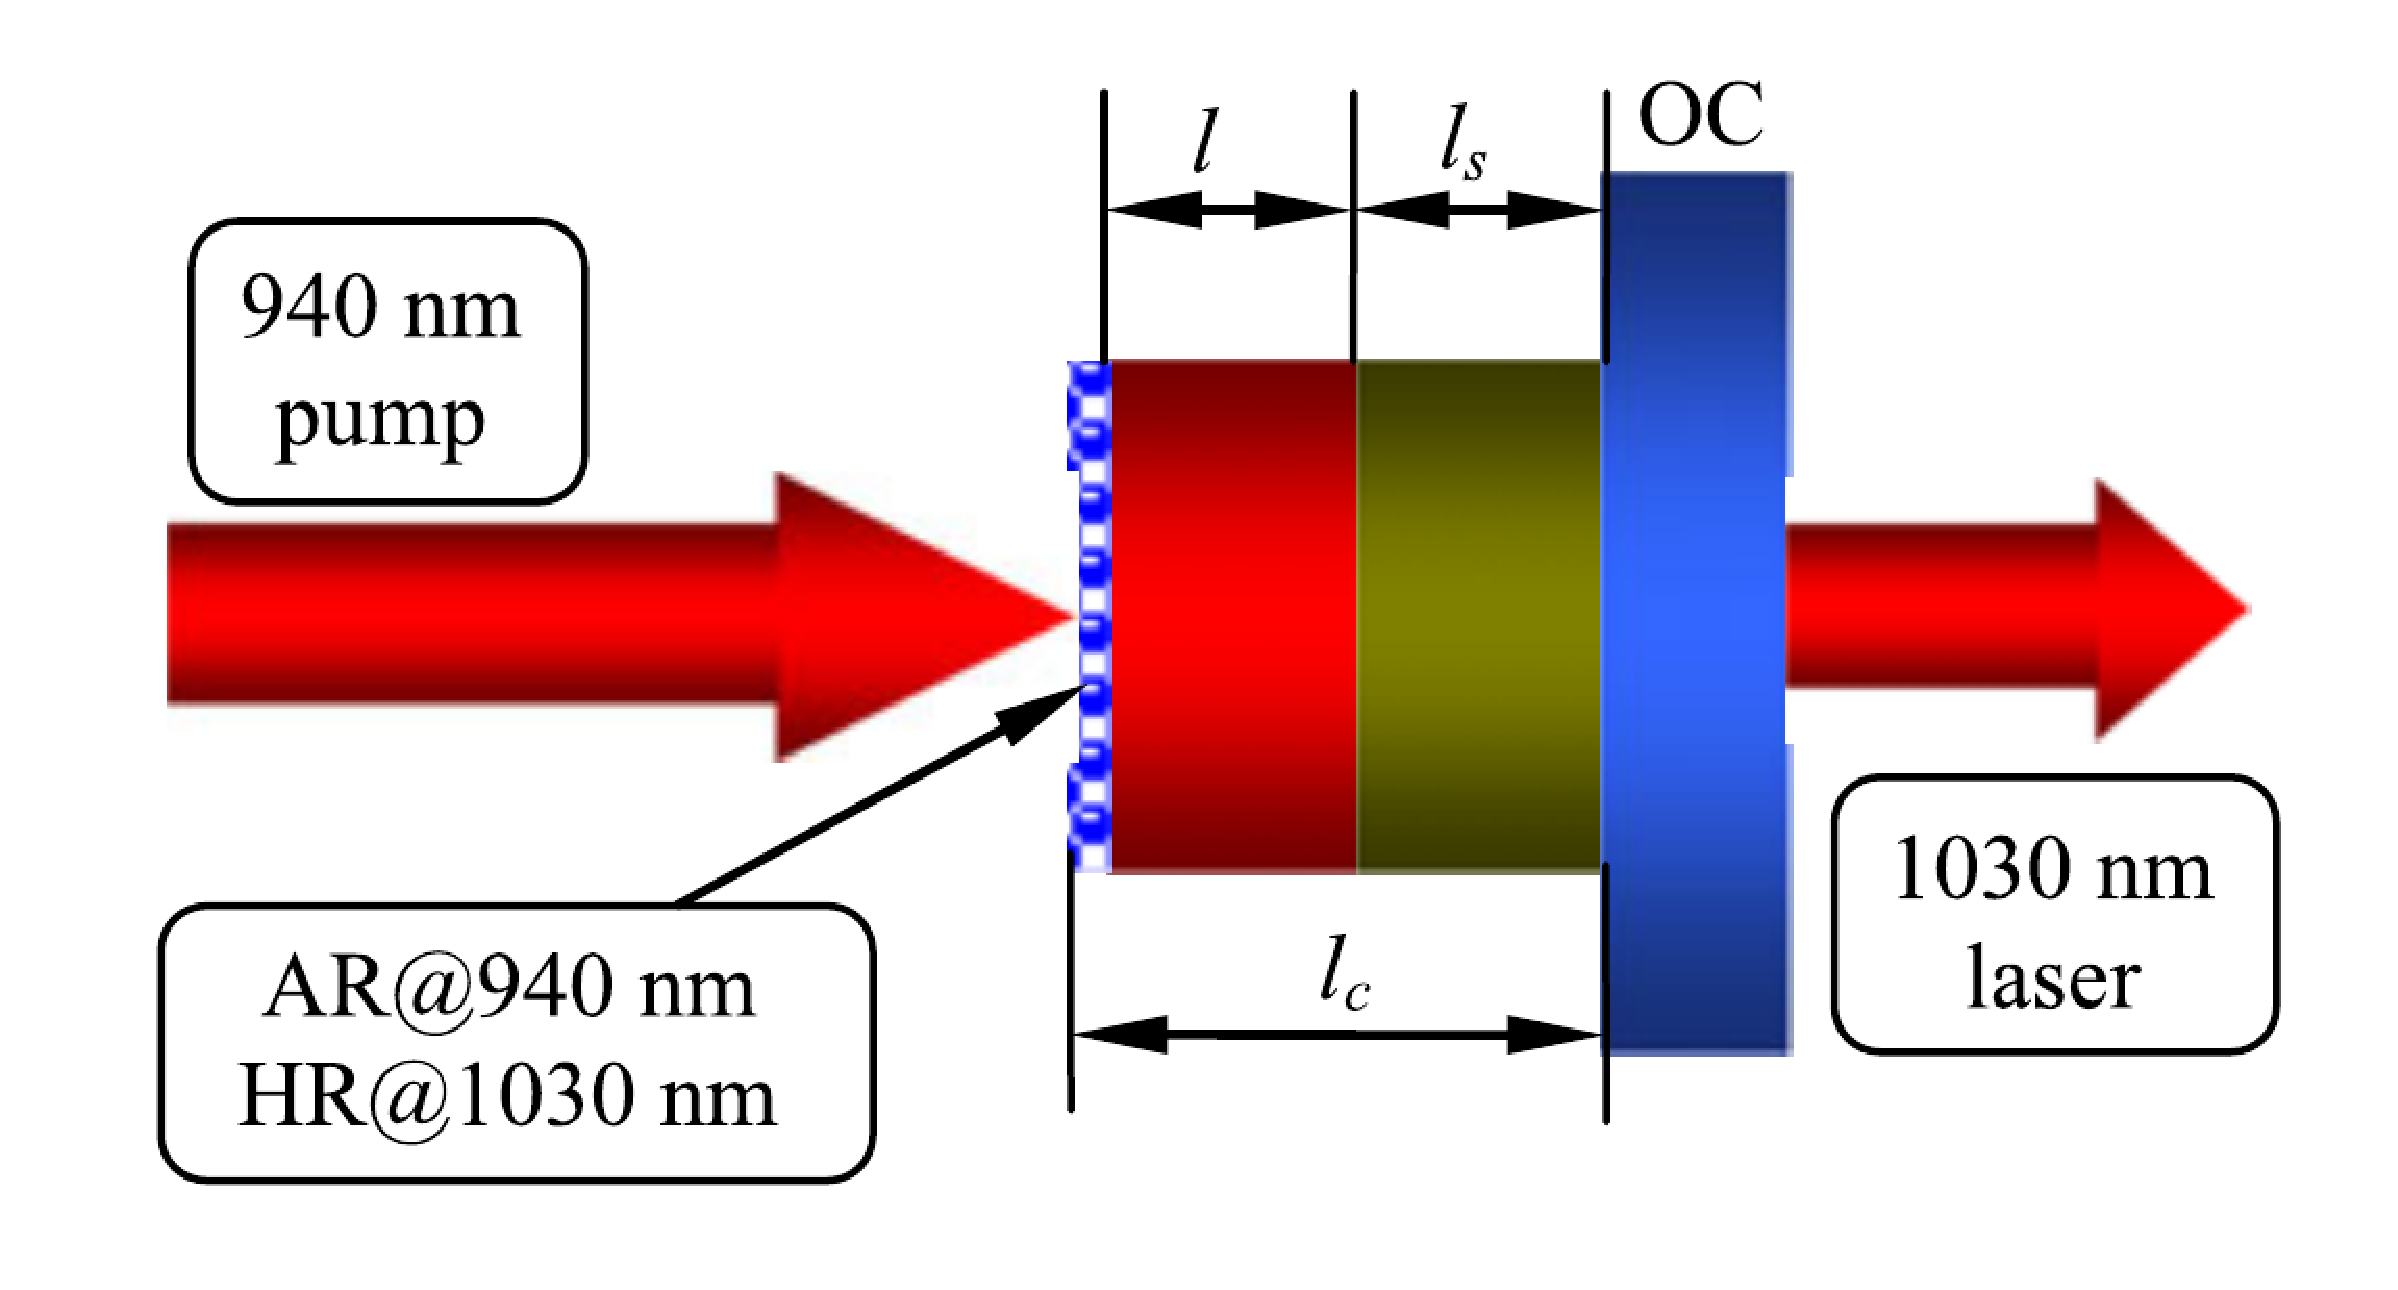
\includegraphics[width=0.55\linewidth]{micro}}
\vspace{1cm} 
\caption{The experimental setup of laser-diode pumped Yb:YAG/Cr:4+:YAG composite ceramics passively Q-switched laser. OC is the output coupler.}
\label{fig:micro} 
\end{figure}

Q-switched microchip lasers also allow the generation of unusually short pulses with durations below 1 ns, in extreme cases even below 100 ps. This holds particularly for passive Q switching with a SESAM [2], but it is also possible to use a saturable absorber crystal e.g. of Cr:YAG or some Cr-doped ceramics [1].

Eventually according to numerical simulation [1,2] the minimum pump power for high-repetition laser system, which is satistied our requrements is quite big > 6-8W this is just for start trigger lasing at 10kHz ( for Nd:YVO4/Cr4+ with best transmission parameters). This is because, optical-to-optical efficiencies – typically of the order of 5-20\%.
At the same time, electrical-to-optical efficiencies sometimes even above 60\%.

Therefore, we are trying to use a laser diode. Fortunately there is powerful high-repetition rate laser diode with quite short pulse duration $\sim 10ns$ at 905 nm from OSRAM Opto Semiconductors (Fig. \ref{fig:osram}).
Despite the fact that the amplification of the detector at this wavelength is small,
the laser power exceeds these losses, moreover at this wavelength the noise is smaller. 
Also it is eye-safe, that expand spectrum of possible applications.

\begin{figure}
\begin{floatrow}
\ffigbox{
\center{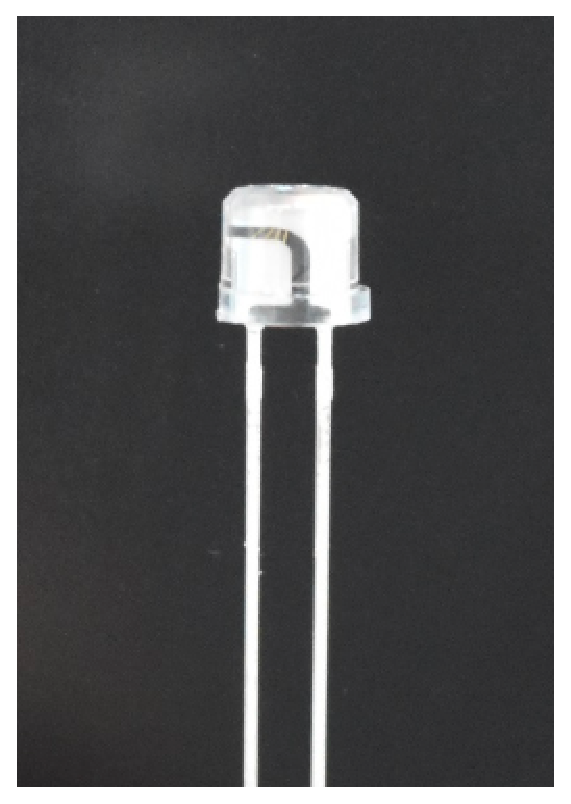
\includegraphics[width=0.45\linewidth]{osram}} 
}{
  \caption{Osram laser diode}%
\label{fig:osram} % or change caption location
}
\capbtabbox{

  \begin{tabular}{|M{4cm}|M{2.5cm}|}
\hline
Peak output power: & \textbf{75 $\pm$ 10 W}  \\ \hline
Forward current: & \textbf{40 A}  \\ \hline
Repetition rate: & \textbf{$\sim$ 100 kHz} \\\hline
Pulse duration: & \textbf{$\geq$ 10 ns} \\\hline
Emission wavelength, $\lambda$: & \textbf{905 $\pm$ 10 nm} \\\hline
Rise time: & \textbf{1 ns} \\  \hline
Fall time: & \textbf{1 ns} \\  \hline
Emmiting area: & \textbf{200 x 10 um} \\  \hline
Beam divergence: & \textbf{25$\pmb{{^\circ}}$ x 9$\pmb{{^\circ}}$} \\  \hline
Operating temperature: & \textbf{-40 .. 100 }$\pmb{{^\circ}}$\textbf{C} \\  \hline
\end{tabular}
}{%
\caption{OSRAM Laser diode characteristics}
\label{tbl:osram_datasheet}
}
\end{floatrow}
\end{figure}





%%%%%%%%%%%% LASER COLLIMATOR SUB-SECTION %%%%%%%%%%%
\subsection{Laser collimator}

Radiation characteristic of laser diode features carries due to its small size, light
quality, low threshold, low cost, these properties the laser diode play an important role in the information time, especially in the field of communication LIDAR.
Optical system is an essential part, which plays an important role in decreasing the divergence angle and homogenizing the beam spot which have an immense
influence on the light signal back from the target.
Together with the detector's collimator, a system with high resolution and high SNR can be obtained.
The design of the system was done by using ZEMAX model which also includes shaping and zooming features of design model.

\begin{figure}[H]
\begin{minipage}[h]{0.52\linewidth}
\center{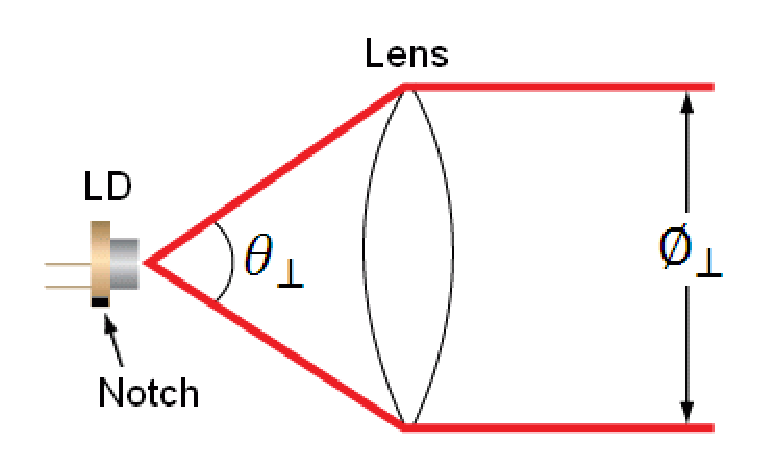
\includegraphics[height=3.15cm, width=0.85\linewidth]{laser_beam_3}} \\ a) 
\end{minipage}
\hfill
\begin{minipage}[h]{0.45\linewidth}
\center{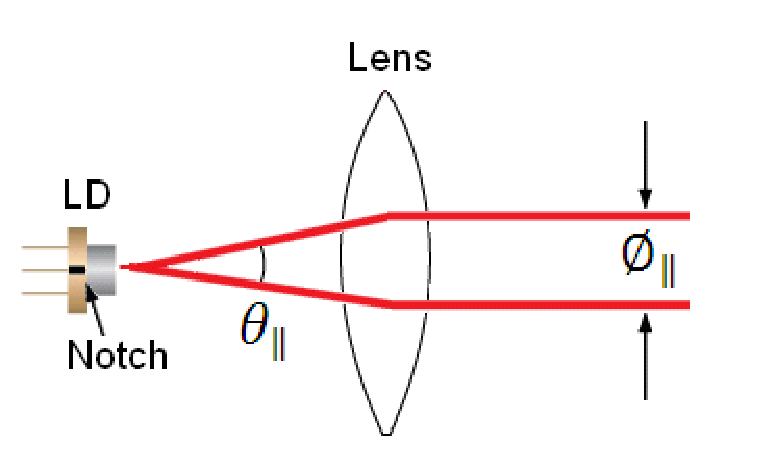
\includegraphics[height=3.25cm, width=1\linewidth]{laser_beam_4}} \\ b)
\end{minipage}
\caption{
In the above schematics, LD denotes the laser diode, \O$_{||}$ and \O$_{\perp}$ are the beam diameters in the parallel and perpendicular orientations, respectively, and $\theta_{||}$
 and  $\theta_{\perp}$ are the divergence angles in the parallel and perpendicular orientations, respectively.\\
a) Perpendicular beam divergence from laser diode.
b) Parallel beam divergence from laser diode.
}
\label{fig:laser_beam}
\end{figure}

The beam divergences of an edge-emitting laser diode will be different in the parallel and perpendicular directions, leading to an elliptical beam (Fig. \ref{fig:laser_beam}).
This can be compensated for by inserting anamorphic prism pairs or cylindrical lenses into the collimated beam, but in our case it's not needed.

Since the output of a laser diode is highly divergent, collimating optics are necessary. 
Traditional spherical lenses have a simple shape that can be
described as an arc of a circle and can be specified using
only a radius of curvature. Although these lenses are simple
to manufacture and inexpensive to use, they suffer in
performance due to a phenomenon called spherical
aberration. This inherent defect is due to the fact that a
spherical shape is not the ideal shape for a focusing or
collimating lens to be. The ideal case is a more complex
shape that is typically defined using a radius of curvature, a
parabolic term (conic), and several high order coefficients.
The complex shape of aspheric lenses allows for correction
of spherical aberration. This provides better quality
collimated beams for collimating applications, a smaller spot
size for focusing applications, and better image quality for
imaging applications. In fact, in many cases just a single
aspheric lens can take the place of several conventional
spherical lenses, leading to a lighter, more compact, less
expensive, and better performing optical system. Aspheres
are now a viable design option for many applications.
Choosing an appropriate aspheric lens for collimating a laser diode is essential, as the resulting beam size and transmission range are dependent on the lens used.

To calculate the beam size of a collimated laser diode, we first need to know its divergences and area of emitting surface.
The specifications for the OSRAM laser diode indicate that the perpendicular and parallel beam divergences are 25${^\circ}$ and 9${^\circ}$, respectively. Because of this asymmetry in the two axes, an elliptical beam will form as the light diverges. To collect as much light as possible during the collimation process, consider the larger of these two divergence angles in any calculations (i.e. 25${^\circ}$).

In paraxial approximation, for beam diameter calculation after passing lens  the following formula is using (Fig. \ref{fig:laser_beam}):

\begin{equation}\label{eq:beam_size}
\text{\O}_{\perp} = 2 \cdot f \cdot \tan{(\frac{\theta_{\perp}}{2})}
\end{equation}

For beam divergence after passing the optical system (Fig. \ref{fig:lens}):



\begin{figure}[H]
\begin{minipage}[h]{0.52\linewidth}
\center{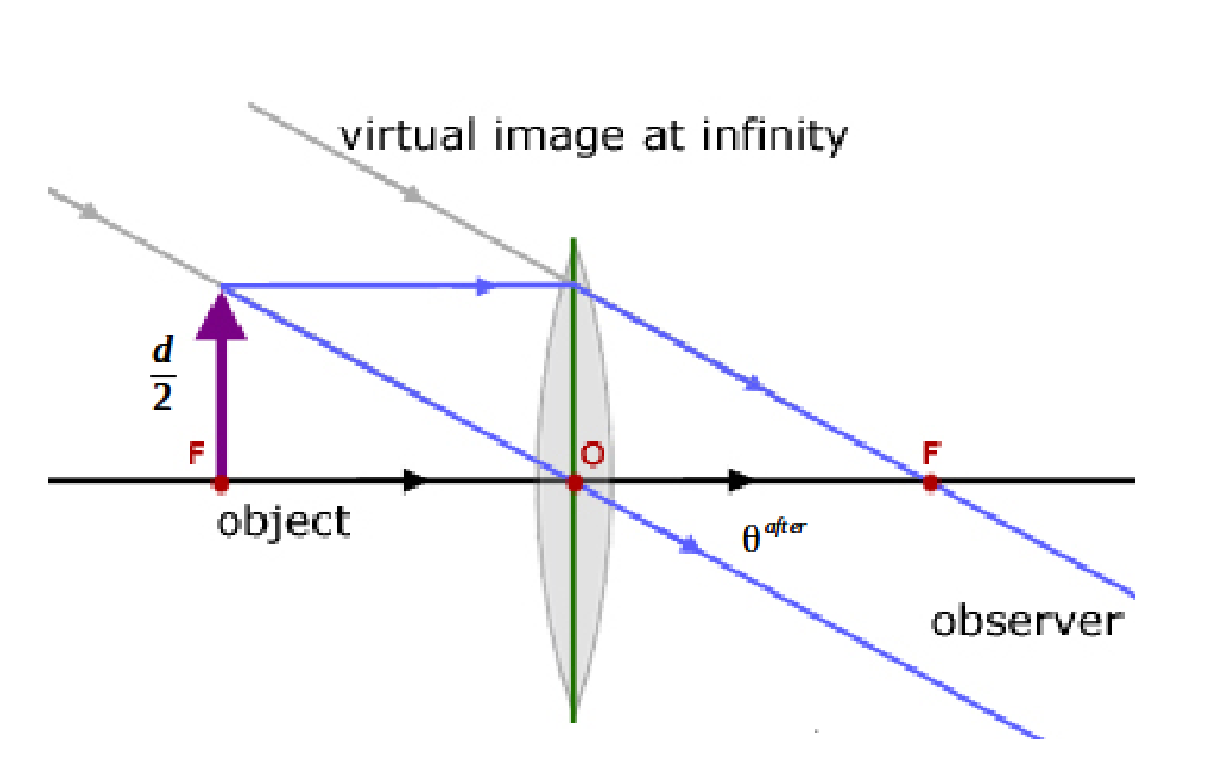
\includegraphics[width=1.2\linewidth]{lens}}
\end{minipage}
\hfill
\begin{minipage}[h]{0.45\linewidth}
\begin{equation}\label{eq:beam_divergence}
\theta^{after} = 2 \cdot \tan^{-1}{(\frac{d}{2f})}
\end{equation}
\end{minipage}
\caption{
Simple demonstration, shows divergence of the beam emitted from object, seated at the focus of the optical system. Here, d is the size of emitting area of laser diode (200 um in our case), f is total focal length of the optical system.
}
\label{fig:lens}
\end{figure}





From the formulas \ref{eq:beam_size} \ref{eq:beam_divergence}, it is obvious that the larger the focal lens, the larger the diameter of the beam and the smaller the beam divergence. It means, that by increasing focal length we can achieve the desirable level of divergence (up to diffraction limit, with assumption we free of aberrations). But, by increasing focal length the beam diameter is also increased.
Since the size of MEMS is only 3.5 mm, we have limitation for focal length (we want reflect all light which are emitted).
The same result can be getting from the Lagrange invariant relationship between the heights and angles of any two rays propagating through the system (in case of linearity of paraxial optics).

Important to note, that even a well-collimated beam has a non-vanishing divergence because of wave-nature of the light, the beam diameter varies (for large distances) with the distance from the laser diode collimator. The resulting beam divergences of the collimated beam:


\begin{equation}\label{eq:beam_divergence}
\theta_{\perp/||} = \frac{2\cdot \lambda}{\pi \cdot \text{\O}_{\perp/||}}
\end{equation}





The simulation results verify the availability that the beam from the
laser diode meets the requirements after optical emission from system.



\subsection{Laser driver}

\noindent\begin{minipage}{0.5\textwidth}
\begin{figure}[H]
% \begin{minipage}[h]{0.52\linewidth}
\center{
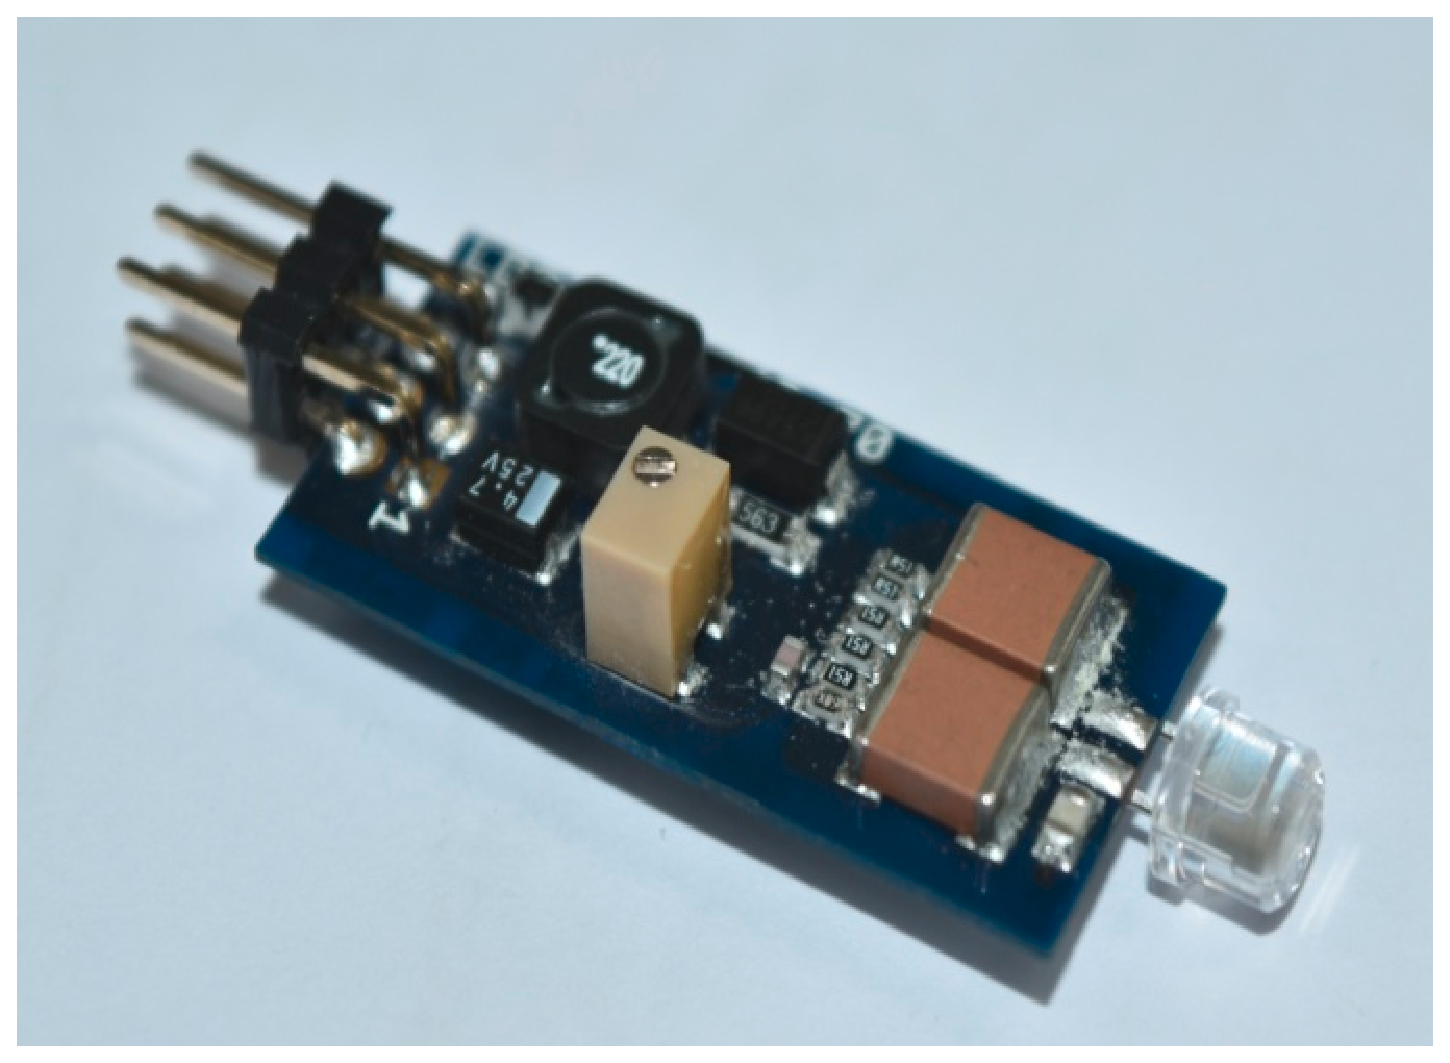
\includegraphics[width=1\linewidth]{laser_driver}
\includegraphics[width=1\linewidth]{laser_output}
} 
\vspace{-3mm}
\caption{Upper fig is laser driver with attached Osram diode. Bottom one is output of detector catched by 2GSa/s oscilloscope after laser shoot. }
\label{fig:laser_driver}
\end{figure}
\end{minipage}
% \vfill
% \begin{minipage}[h]{0.52\linewidth}
% \center{\includegraphics[width=1\linewidth]{laser_output}} \\b)
% \end{minipage}
% \end{minipage}
\hfill
\begin{minipage}{0.4\textwidth}
To operate Osram laser diode the laser driver is required. The simple one is shown in the upper part in Fig \ref{fig:laser_driver}.
This is commercial one, provides 40A at repetition rate up to 100kHz(?).
The lower part shows the screenshot of the 2Gsa/s oscilloscope, as can be seen, the pulse duration is of the order of 10 ns. The detector was SiPM which is described in the next section.

Our team made an analog of this laser driver, smaller in size with the same characteristics, as well as with a combined detector (SiPM) part. 

\subsection{Final}
Finally we got laser system with the following params:
*table*


% \end{minipage}
\end{minipage}

